%\section{Grundlagen, Stand der Forschung}
% infromieren what quarter- / halfwaveplate und polarizer are
% - Halfwaveplates:
%   Rotate Polarisation
% - Quarterwaveplates:
%   Turn linear to circular polarization

\section{Grundlagen}
In diesem Kapitel wird das notwendige Wissen für die vorliegende Arbeit vermittelt. Es werden Grundlagen über die Administration bezüglich Softwareentwicklung als auch Methoden zum Programmieren von Programmen für die Entwicklung einer Software beschrieben.\\

\subsection{Agile Software-Engineering}
Die Software wurde mit einer teils Agilen Software Entwicklungsmethode realisiert. Der Ansatz der agilen oder auch inkrementelle Softwareentwicklung wurde aus Gründen der Zusammenarbeit mit dem Kunden(Empfänger und Nutzer des Softwareproduktes) entwickelt. Durch die inkrementelle Auslieferung an den Kunden, hat dieser die Möglichkeit neue Funktionen spontan anzubringen und des dem Kunden der spontanen Änderung der Software ausgewählt. Daneben ist die agile Softwareentwicklung geeignet für kleine Software und kleinere, flexible Kunden.

Trotzdem wurden die Anforderungen im Vorhinein definiert und werden nicht abgeändert. Daraus resultiert eine eher vermischte Methode, die sogenannte plangesteuerte und agile Entwicklung. Dabei werden Iterationsschritte lediglich in den einzelnen Projektphasen zugelassen und verändern nicht die gesamte Struktur des Projektes. Jedoch ist es trotzdem möglich Änderungen in der Anforderungsspezifikation vorzunehmen, wenn dies in der Entwurfs- und Implementierungsphase detektiert wird. In grösseren Projekten werden die Phasen Entwurf und Implementierung getrennt. In kleineren Projekten wie diesem, verschmelzen diese Phasen und alle anderen Aktivitäten werden in diesem Prozess integriert. Programme sollen mit einer guten Softwarepraxis entwickelt werden, damit diese Wiederverwendung finden und diese gut zu Unterhalten sind. Dazu sollen sie für den Ersteller und andere Programmierer:innen nachvollziehbar sein.
Verbesserungen können in der Regel schnell implementiert werden. Dazu fällt das akribische Dokumentieren und Planen im Vorfeld weg. Dies hat für den Empfänger und für die Entwickler einen grossen Vorteil. [6] % S. 214;
Zusätzlich konnte für dieses Projekt Open-Source-Software, also frei zugängliche Software genutzt werden. So wurde eine API von Meerstetter Engineering für die Kommunikation mit dem TEC-Kontroller verwendet.
% \textit{Commercial Off-the-Shelf, COTS}: bereits fertiges System, das mit wenigen Anpassungen einsatzbereit ist (Meerstetter MeCom API) aber kostenlos erhältlich -->

\subsection{Wiederverwendbarkeit von Software $-$ Objektorientiertes Programmieren OOP}
Um die Software effizienter gestalten zu können wurde oft auf die Wiederverwendbare von Software dritter zugegriffen. So wurde z.B. die Kommunikation mit dem TEC-Kontroller erstellt. Den Code für die Kommunikation mit dem TEC-Kontroller wurde von Meerstetter Engineering zur Verfügung gestellt.
Für die graphische Benutzeroberfläche wurde das Framework von \textit{Customtkinter} und \textit{Tkinter} und für die Darstellung der Graphen wurde das Framework \textit{Matplotlib} verwendet.\\
Daneben wurde soweit es ging Objektorientiertes Programmieren eingesetzt. Dies vereinfacht die Übersicht des Programmcodes massiv.

\subsection{Entwurfsmuster - Design Patterns}
Für die Programmierung der Steuerung wurde ein sogenanntes \textit{Design Pattern} verwendet. Design Patterns sind verallgemeinerte vordefinierte Programmiermethoden und Softwarearchitekturen, die für gewisse Fälle in der Softwareentwicklung erdacht wurden. Sie sind dazu da wiederkehrende Probleme in der Softwareentwicklung mit einer geeigneten spezifischen Methode zu lösen. Daneben ermöglichen sie eine einfache Handhabung mit Daten, Infrastrukturen, Anzeigen und der Erweiterung und Abänderung des Programmcodes zu jeder Zeit und ohne anderen Code drastisch zu verändern. Unter den Design Patterns gibt es wiederum verschieden Kategorien, die die Einsatzgebiete der Design Patterns beschreiben. Grundsätzlich jedoch werden die Beschreibungen der Patterns in vier Hauptelemente unterteilt. Der Name, das Problem, die Lösung und die Konsequenz beim Verwenden des Musters. Für die Steuerung wurde das \textit{Producer - Consumer} - Design Pattern verwendet, weiteres mehr in Abschnitt \ref{section:_producer_consumer} $[7]$

% [https://medium.com/@amirm.lavasani/design-patterns-in-python-a-series-f502b7804ae5]

\subsection{Parallelität / Gleichzeitigkeit im Programm}
Das Lesen der Daten auf dem TEC-Controller und das Anzeigen der Daten in der Benutzeroberfläche sind zwei Prozesse. Weil ein Prozessor in einem Computer Informationen nur seriell verarbeiten kann, ist es nicht möglich mit einem synchronen Programm die geforderten Aufgaben abzuarbeiten. Der  inaktive Prozess würde nicht laufen, die Aufgabe würde somit nicht ausgeführt. Zeigen kann sich dieser Effekt, wenn die Anzeige einfriert. Die Aufgaben für die Steuerung müssen also asynchron oder parallel abgearbeitet werden. Um dieses Problem zu bewältigen, gibt es drei Programmiermethoden, die ein Programm in verschiedene \textit{Pfade oder Aufgaben} aufteilt. Asynchrones programmieren, \textit{Threading} oder die Multiprozessorprogrammierung, wobei asynchrone Abläufe und \textit{Threading} sehr ähnlich sind. In den Illustrationen gezeigt werden die Unterschiede der Methoden.

\begin{figure}[H]
    \centering
    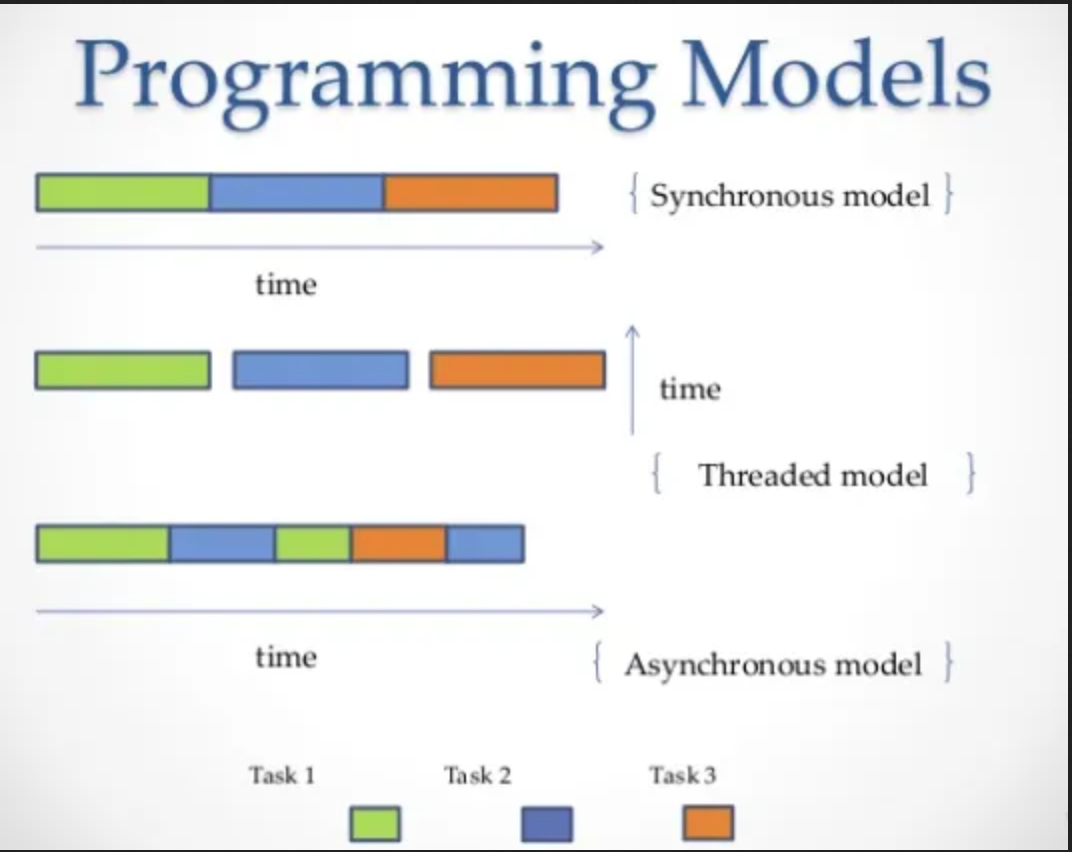
\includegraphics[scale=0.6]{98_images/threading_asynchronous.PNG}
    \caption{In der Abbildung sind die Unterschiedlichen Arbeitsweisen der verschiedenen Programmiertechniken gezeigt.}
    \label{fig:multi_threading_async}
\end{figure}

\begin{table}[H]
    \centering
    \begin{tabular}{|l|c|c|c|}
         $-$&Asynchron &Threading &Multiprozessor\\
         Standard&Ja &Ja  &Ja\\
         Komplexität &Simpel &Fortgeschritten &Komplex\\
         Nutzen &Ja &Ja &Ja
    \end{tabular}
    \caption{In der Tabelle sind verschiedene Methoden, um Programme asynchron oder parallel ablaufen zu lassen. Asynchron und \textit{Threading} sind ähnlich, die Multiprozessormethode ist eine fortgeschrittene Programmiertechnik.}
    \label{tab:async_threading_multiprocessor}
\end{table}

Bei der asynchronen Methode und beim \textit{Threading} werden vom einen Prozess Aufgaben ausgeführt, wenn ein anderer Prozess eine Wartezeit durchläuft. Dies ist immer der Fall, wenn ein Prozess den Prozessor des Computers nicht verwendet, dann kann ein anderer Prozess den Prozessor nutzen. Beim Multiprozessor werden die parallel auszuführenden Aufgaben auf verschiedene Prozessoren aufgeteilt, verhindern sich somit nicht direkt. Die Schwierigkeit jedoch ist die Datenintegrität zu gewährleisten. Alle getrennten Prozesse müssen zur richtigen Zeit mit der korrekten Datengrundlage arbeiten können, woher weiss Prozess A, dass die Daten auf dem gemeinsam genutzten Speicher fertig verarbeitet sind? $-$ Neben andernen Herausforderung bei der Multiprozessor Programmierung, stellt dies die grösste Herausforderung dar. $[]$

% https://medium.com/velotio-perspectives/an-introduction-to-asynchronous-programming-in-python-af0189a88bbb

\subsection{Serielle Kommunikationsschnittstelle - USB}
Für die Übertragung der Daten wurde das USB Protokoll verwendet. Der TEC-Controller kann so direkt an den Raspberry PI angeschlossen werden und die API der Herstellerfirma Meerstetter, kann auch direkt verwendet werden. Diese Schnittstelle erwies sich währen der Test als stabil.

% Und noch schnell die ganze Bibliographie zitieren:
\nocite{*}